\documentclass[10pt]{beamer}
\usetheme{Rochester}
\usepackage[utf8]{inputenc}
\usepackage{amsmath}
\usepackage{amsfonts}
\usepackage{amssymb}
\usepackage[export]{adjustbox}
\setbeamertemplate{footline}[frame number]
\author{Justin Anguiano}
\title{Performance Optimization}
%\setbeamercovered{transparent} 
%\setbeamertemplate{navigation symbols}{} 
%\logo{} 
%\institute{} 
%\date{} 
%\subject{} 
\begin{document}

\begin{frame}
\titlepage
\end{frame}

%\begin{frame}
%\tableofcontents
%\end{frame}

\begin{frame}{}
Goal --- Improve Physics analysis performance \\
\quad \quad \\
Use different C/Python approaches to obtain a low programming overhead but high performance\\ 

\quad \quad \\
Today: a look at multithreading and multiprocessing in C++ ROOT
\end{frame}

\begin{frame}
\begin{columns}
	\begin{column}{0.5\textwidth}
\scriptsize
   		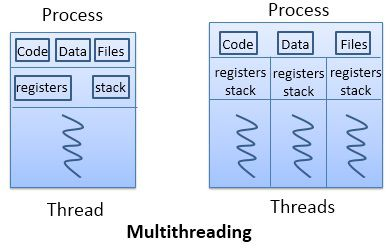
\includegraphics[scale=0.45, left]{Multithreading.jpg}\\
   		\textbf{Multiprocessing}-\\
   		\begin{itemize}
   			\item adds CPUs to increase performance
   			\item processes run concurrently
   			\item creating/managing processes is resource intensive
   			\item processes do not share memory
   		\end{itemize}
   		\textbf{Multithreading}-\\
   		\begin{itemize} 
   			\item adds threads to a single CPU to increase performance
   			\item multithreading is economic for the system
   			\item threads share memory
   		\end{itemize}

\end{column}
	\begin{column}{0.5\textwidth}
	Definitions:\\
	\scriptsize
	\textbf{thread} of execution is the smallest sequence of programmed instructions that can be managed independently by a scheduler\\
	The number of threads possible depend on the number of cores in the CPU\\
	\quad \quad \\
	
	\textbf{process} is the instance of a computer program that is being executed by one or many threads\\
\end{column}
\end{columns}
\scriptsize
\quad \quad \\
There are parallelization tools to exploit both of these approaches built into root!
\end{frame}

\begin{frame}{Test 1: Local multi-threading}
\textbf{Task to be optimized: Read File(s) containing a TTree, produce histograms from elements of the tree(s), write histograms to a TFile}\\
\quad \quad \\
\scriptsize
\textbf{ Three histograms are produced: TH1D: track $p_{T}$ weighted by $1/p_{T}$, TH1D: track $p_z$, TH2D, track $p_x$ vs $p_y$} \\
\normalsize
\quad \quad \\
First attempt using ROOT6 parallelization on local machine (laptop)\\
methods:\\
\begin{itemize}
\item Sequential run over a test file with TTreeReader (Compiled and Interpreted)
\item Parallelized run over a test file with TTreeReader (Compiled and Interpreted)
\end{itemize}

Test File Details\\
\begin{itemize}
\item code adapted from example: \url{https://root.cern.ch/doc/v612/imt101__parTreeProcessing_8C.html} 
\item uses fake event file containing 48,000 events; each with some number of tracks per event
\item total tracks overall $\approx 2.4e+7$ 
\end{itemize}

\end{frame}


\begin{frame}{Test 1: Local multi-threading}
First Test Results:\\
\begin{columns}
	\begin{column}{0.5\textwidth}
	\begin{itemize}
		\scriptsize
		\item Time is Mean time $\pm$ stdev over 10 trials
		\item no guarantee of system releasing requested resources (nthreads) so perform multiple trials
		\item data point at nThreads = 0 is the basic sequential program
		\item high threadcount performance possibly bottlenecked by system?
		\item Takeaway: Compiling is important! $\approx $Factor of 2 improvement
	\end{itemize}
	\end{column}
	\begin{column}{0.5\textwidth}
   		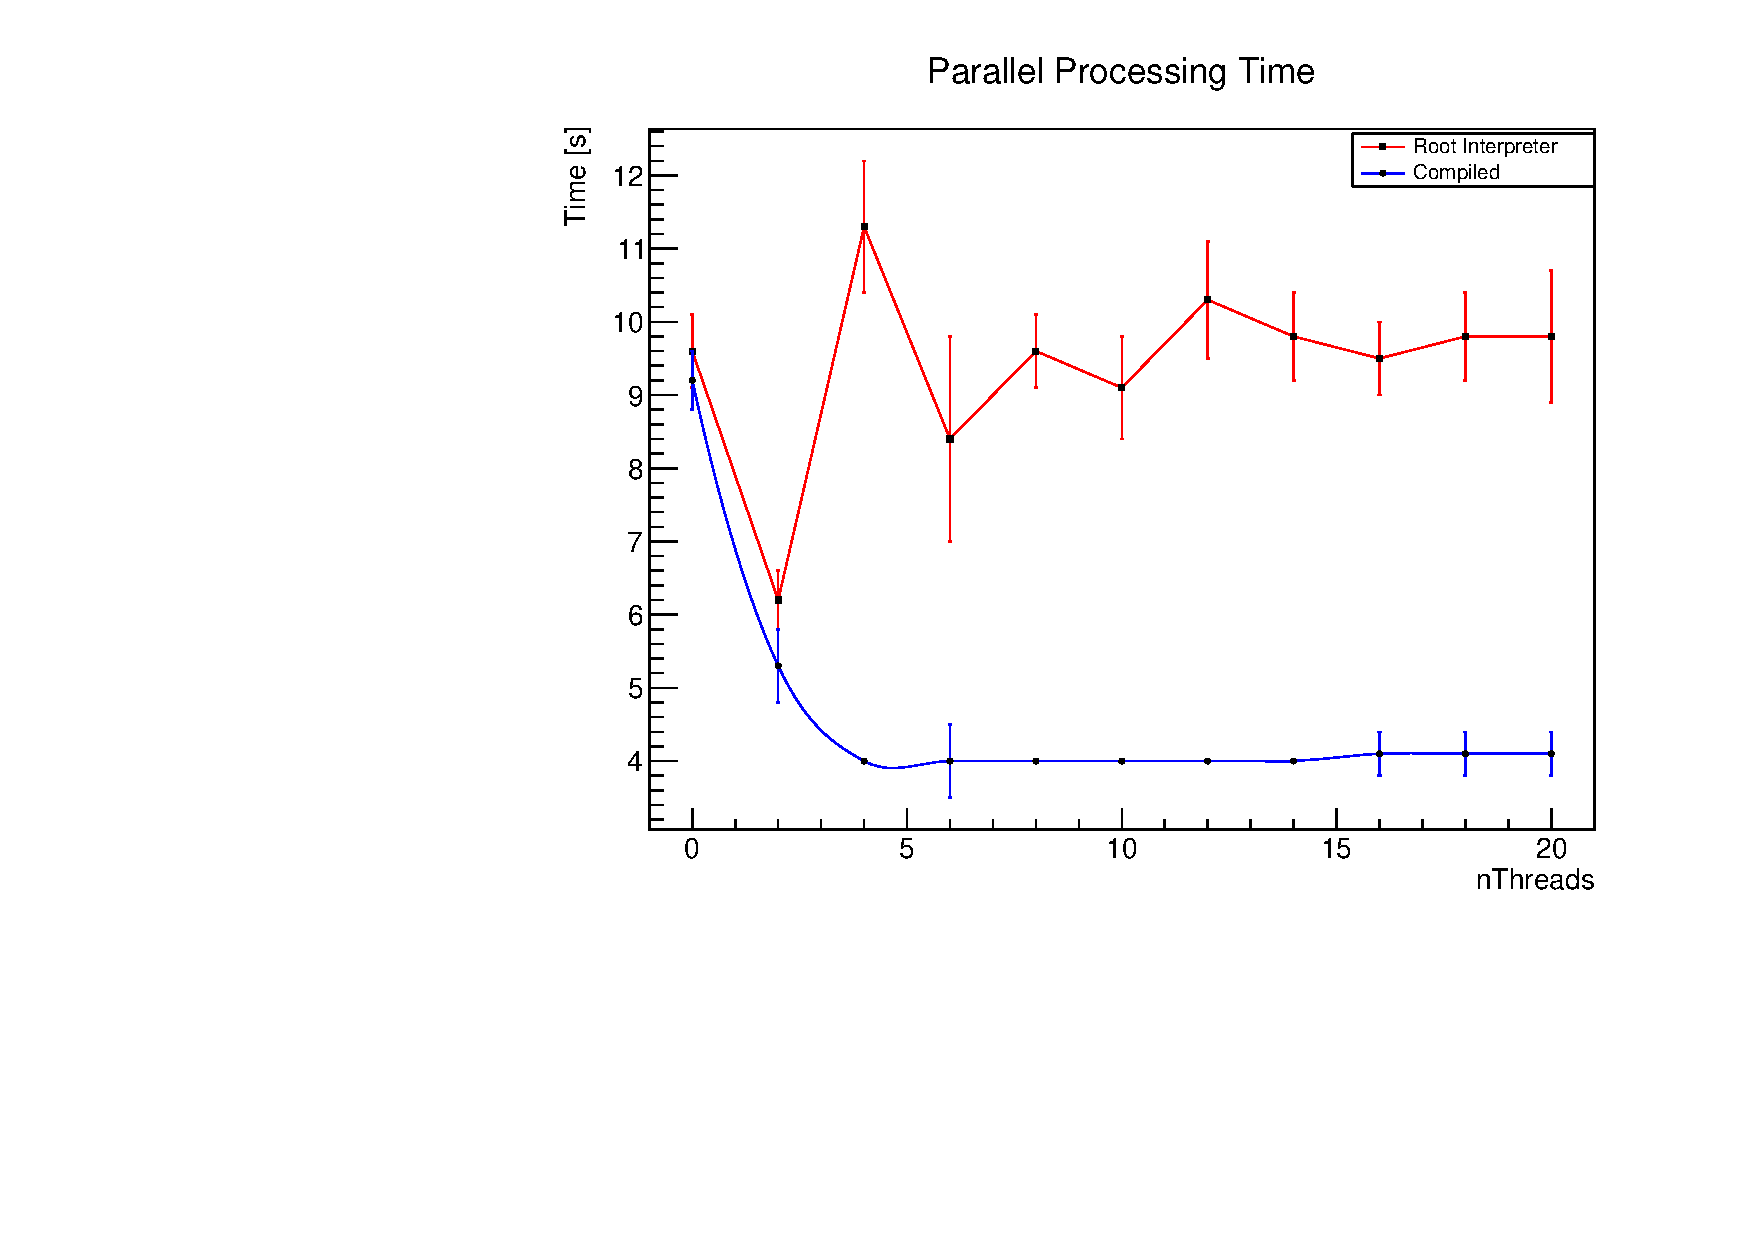
\includegraphics[scale=0.3, left]{../ParTree/test1plot.pdf}

	\end{column}
\end{columns}
\end{frame}

\begin{frame}{Test 2: UNL multi-threading}
Second attempt using ROOT6 parallelization versus classic(Make Class) sequential program (my current approach) on  t3.unl.edu\\
Methods:\\
\begin{itemize}
\item Sequential run over multiple test files with TTreeReader (Compiled Only)
\item Parallelized run over multiple test files with TTreeReader (Compiled Only)
\item Sequential run over multiple test files with MakeClass (Compiled and Interpreted)
\end{itemize} 

Test File set Details:\\
\begin{itemize}
\item using 9 files from Dataset: \url{/SingleMuon/Run2018D-PromptReco-v2/AOD }
\begin{itemize}
\tiny
	\item Physics group: NoGroup Creation time: 2018-08-01 13:16:41 Status: VALID Type: data Dataset size: 150070502441346 (150.1TB) Number of blocks: 267 Number of events: 511823047 Number of files: 45330 
	\end{itemize}
\normalsize
\item 1,576,737 events each with at least 1 conversion per event
\item total tracks overall (exactly 2 per conversion) = 14,190,956   
\end{itemize}

\end{frame}

\begin{frame}{Test 2: UNL multi-threading}
File Sequence Details:\\
\begin{columns}
	\begin{column}{0.5\textwidth}
\scriptsize
\begin{itemize}
    \item \url{Run2018_100.root} 
         \begin{itemize}
         	\scriptsize
      		\item   contains 193388 events
       		\item  contains 1547322 unique conversion tracks
        \end{itemize}
   \item \url{Run2018_110.root}
        \begin{itemize}
        \scriptsize
     		 \item   contains 140502 events
     		\item   contains 950444 unique conversion tracks
        \end{itemize}
   \item \url{Run2018_120.root}
        \begin{itemize}
        \scriptsize
      		 \item  contains 99085 events
      		 \item  contains 602330
        \end{itemize}
    \item \url{Run2018_130.root} 
        \begin{itemize}
        \scriptsize
       		\item  contains 62289 events
       		\item  contains 347156 unique conversion tracks
        \end{itemize}
   \item \url{Run2018_141.root}
        \begin{itemize}
        \scriptsize
      		\item  contains 218339 events
       		\item  contains 1958272 unique conversion tracks
        \end{itemize}
        \end{itemize}
        \end{column}
        \begin{column}{0.5\textwidth}
	\scriptsize
		\begin{itemize}
   \item \url{Run2018_155.root}
        \begin{itemize}
        \scriptsize
      		\item   contains 269483 events
      		\item   contains 2968340 unique conversion tracks       
        \end{itemize}
   \item \url{Run2018_166.root}
        \begin{itemize}
        \scriptsize
      		 \item  contains 172409 events
       		\item  contains 1299172 unique conversion tracks
        \end{itemize}

    \item \url{Run2018_176.root}
        \begin{itemize}
        \scriptsize
      		\item   contains 127117 events
      		\item   contains 832024 unique conversion tracks
        \end{itemize}
    \item \url{Run2018_193.root}
        \begin{itemize}
        \scriptsize
      		 \item  contains 294125 events
       		\item  contains 3685896 unique conversion tracks 
        \end{itemize}
\end{itemize}
\end{column}
\end{columns}

\end{frame}

\begin{frame}
First Cluster Test Results:\\
\tiny
(Using full 9 file dataset)\\
\begin{columns}
	\begin{column}{0.5\textwidth}
	\begin{itemize}
		\scriptsize
		\item Time is Mean time $\pm$ $s/\sqrt{N}$ over 5 trials
		\item data point at nThreads = 0 is the basic sequential program
		\item high threadcount again not optimal, chokes up the system
		\quad \quad \\
		\item Classic sequential approaches using MakeClass (Compiled and Interpreted)--
			\begin{itemize}
				\scriptsize
				\item $265.4 \pm  9.2$ [s] (Interpreted)
				\item $171.0 \pm  10.6$ [s] (Compiled)

			\end{itemize}
			\quad \quad \\
		\item ROOT6 mutlithreading is very good!
	\end{itemize}
	\end{column}
	\begin{column}{0.5\textwidth}
   		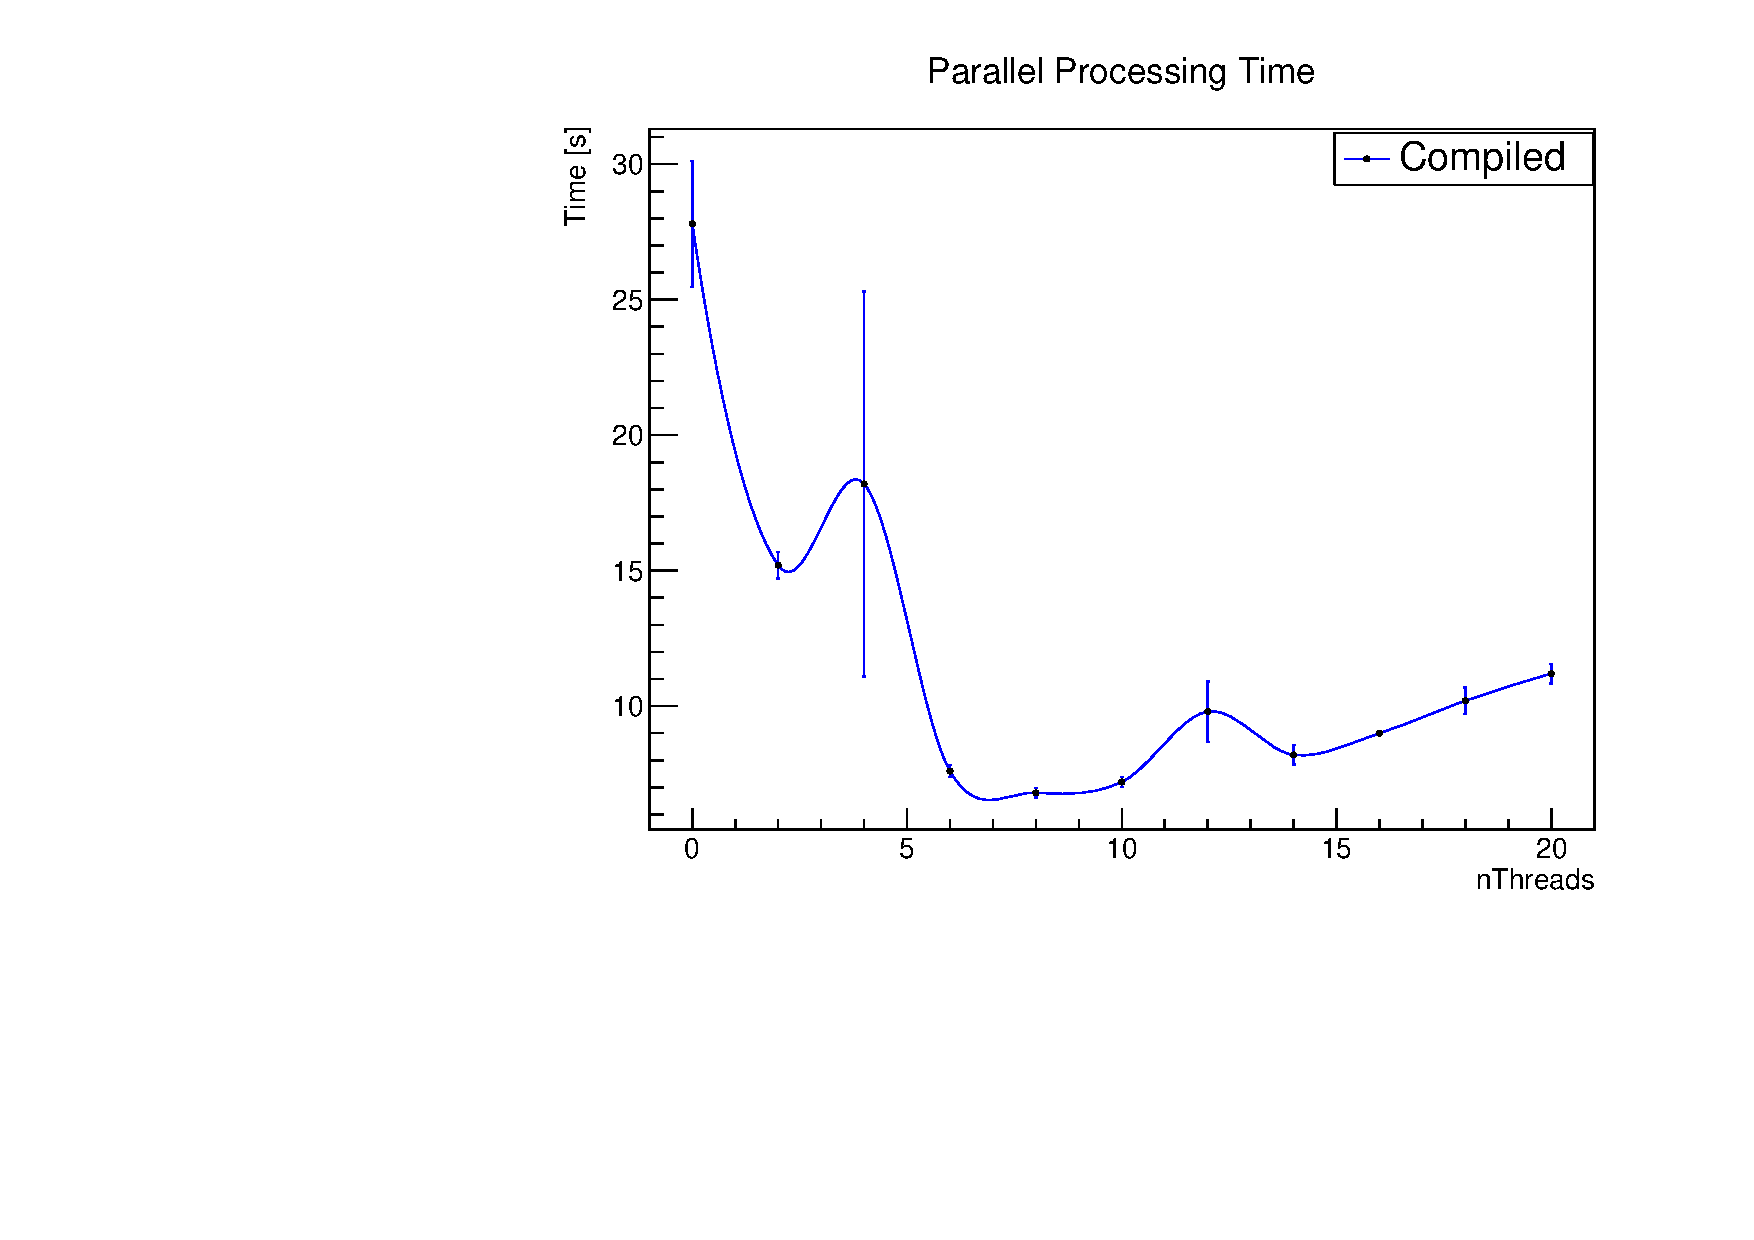
\includegraphics[scale=0.3, left]{../ParTree_t3/test1plott3.pdf}

	\end{column}
\end{columns}

\end{frame}

\begin{frame}{Test 2: UNL multi-threading}
Second Cluster Test:The impact of data size on performance\\
\begin{columns}
	\begin{column}{0.5\textwidth}
		\scriptsize
	\begin{itemize}
		\item Time is Mean time $\pm$ $s/\sqrt{N}$ over 5 trials
		\item nTracks is the accumulated number of tracks looped over for a given number of files that are run in a preserved order
		\item Parallel is run with the previously optimal number of threads (8)
		\item Parrellization is faster and more consistent at any size of dataset 
		\item As data gets larger the parallel benefit becomes more significant
	\end{itemize}
	\end{column}
	\begin{column}{0.5\textwidth}
   		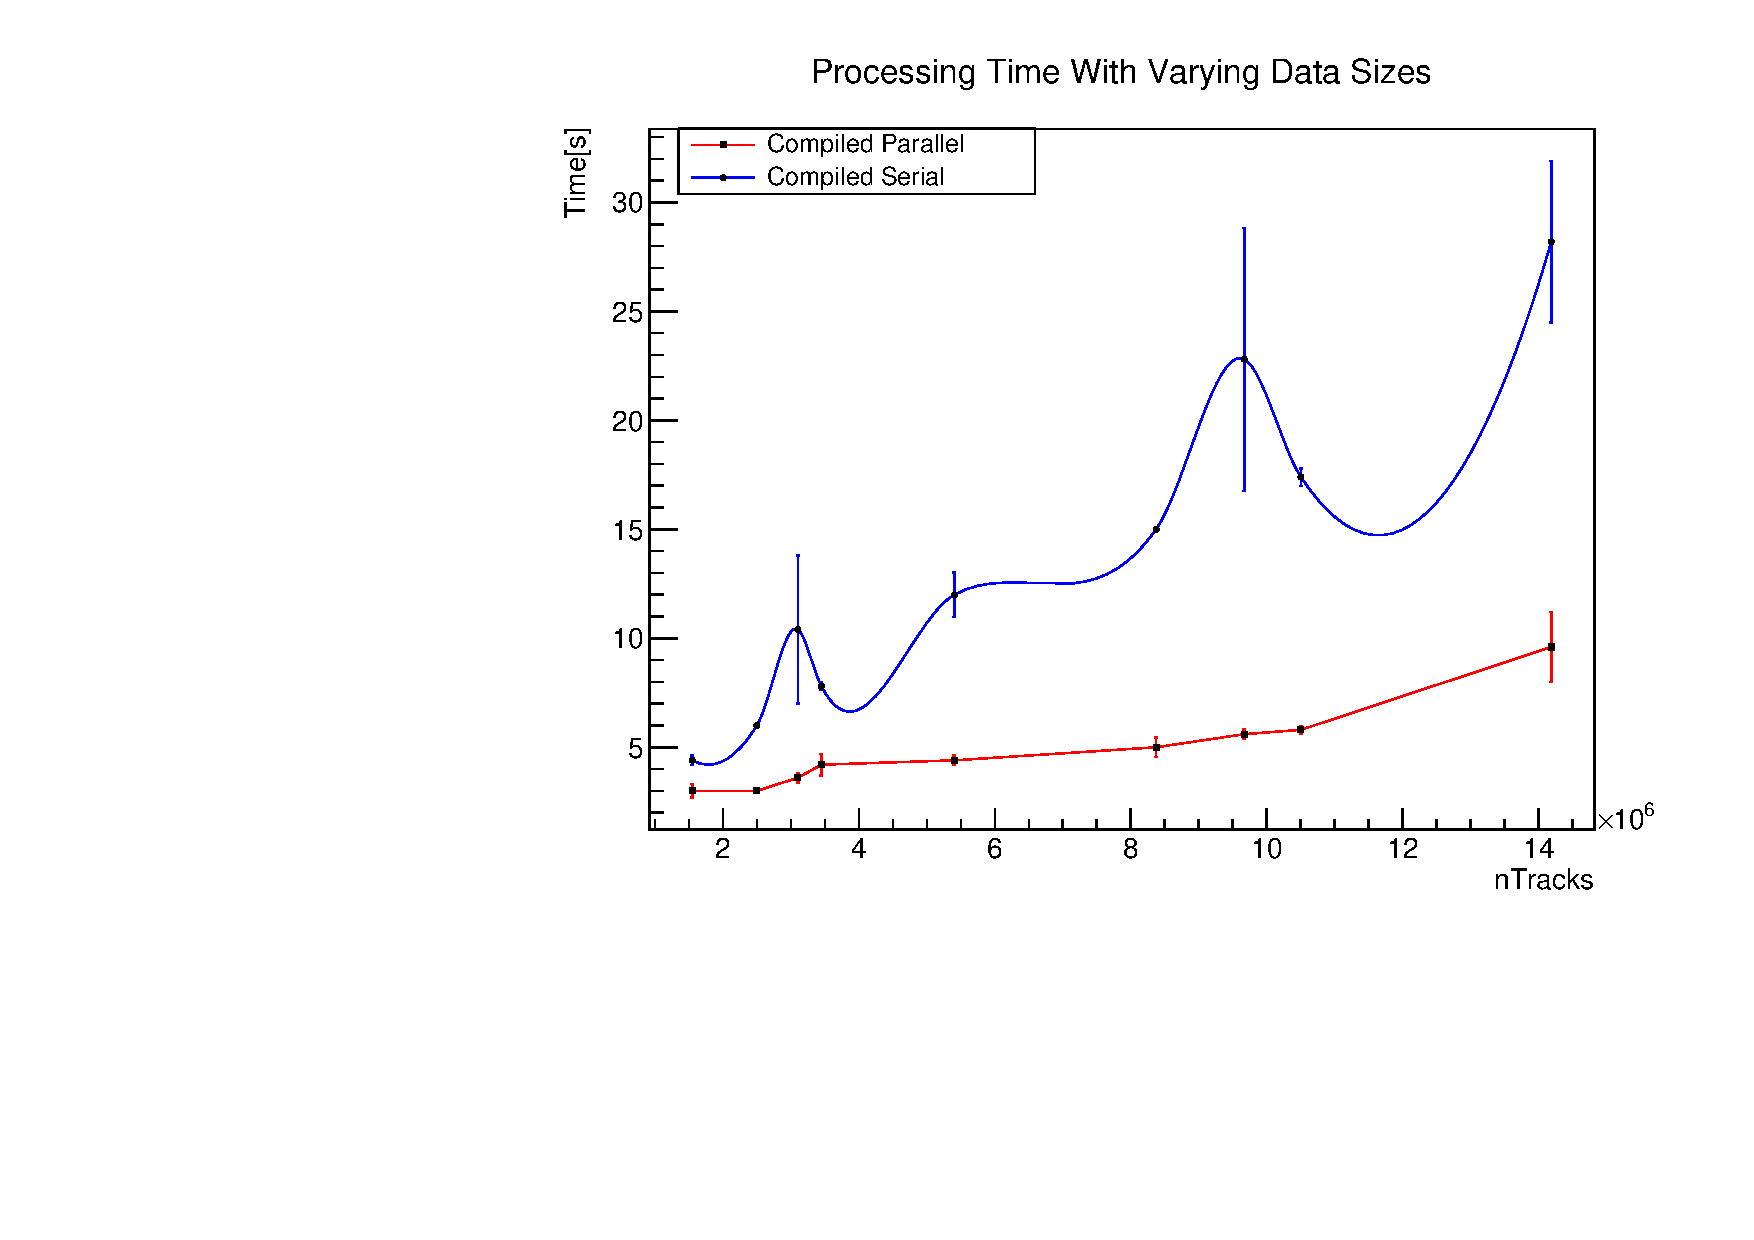
\includegraphics[scale=0.3, left]{../ParTree_t3/sizetestt3.pdf}
	\end{column}
\end{columns}

\end{frame}


\begin{frame}{Test 3: UNL multi-processing}
Two ``new" tools:\\ 

\textbf{Parallel ROOT Facility (PROOF)} and \textbf{Selectors}\\
\quad \quad \\
PROOF and Selector are designed be be used together\\
PROOF is a toolset used to manage/delegate processes between nodes on a cluster\\
Selector is the ROOT6 version of a MakeClass i.e. TTreeReaderValues/Arrays\\
\quad \quad \\
Using them is easy:
\begin{itemize}
\item write a simple analysis in Selector
\item load all input files into a TChain
\item create a PROOF instance
\item tchain.Process(``selector.C")
\end{itemize}


\end{frame}
\begin{frame}{Test 3: UNL multi-procesing}
Test 3: compare multiprocessing and multithreading at UNL\\
\quad use the same 9 files with the same task\\
\quad also try a large 918 file (Single Muon) test case with the same task\\

\quad \quad \\
the large dataset contains 146,607,893 events

\quad \quad \\
\begin{tabular}{|c|c|c|c|}
\hline 
Method & numFiles & nTrials & Time (s) \\ 
\hline 
multiThread & 9 & 5 & $6.8 \pm 0.2$\\ 
\hline 
multiProcess & 9 & 3 & $92.3 \pm 0.9$ \\ 
\hline 
\hline
\hline 
multiThread & 918 & 1 & 26m 4s \\ 
\hline 
multiProcess & 918 & 1 & 126m 56s \\ 
\hline 
\end{tabular} \\
\quad \quad \\ 

\quad \quad \\
Multithreading is still significantly faster!!\\
Process resource and management overhead is high\\
Possible to combine Multiprocessing + Multithreading in ROOT??\\ In principle yes..
\end{frame}

\begin{frame}{Application to SUSY Analysis}
New tool availble at github : githublink.com\\
Basic Analysis template -- good for any Tree reading + Histogram producing analysis\\
Modular tools assembled to automatically parse Trees and perform multithreading $\rightarrow$  just make histograms!

\quad \quad \\
How it works:
\begin{itemize}
\item uses a Python script for input interface
	\begin{itemize}
		\scriptsize
		\item just feed in a list of signal or background rootfiles with the treename 
	\end{itemize}
\item uses a TSelector to access all possible TTreeReaderValue branches in analysis
	\begin{itemize}
	\scriptsize
		\item easily automatically generated with just tree.MakeSelector("myselector")
	\end{itemize}
\item histset.c is the meat of the analysis, contains threaded histograms and physics analysis code
	\begin{itemize}
		\scriptsize
		\item this is the only place where code needs to be modified
	\end{itemize}
\item the custom class ParTreeProcessing.c manages the selector/multithreading/histograms
\end{itemize}
\end{frame}

\begin{frame}{Application to SUSY Analysis}
Test 4: Multithreaded SUSY Analysis
Running over all large backgrounds and two signal trees\\
\quad \quad \\
Background: (all HT binned)\\
\url{DYJetsToLL_HT.list}\\
\url{QCD_HT.list}  \\
\url{TTJets_HT.list} \\ 
\url{WJetsToLNu_HT.list}\\  
\url{ZJetsToNuNu_HT.list} \\

\quad \quad \\
Signal: \\
\url{SMS_TChiWZ_ZToLL.list}\\    
\url{SMS_300_75} and \url{SMS_175_135}\\

\end{frame}

\begin{frame}{SUSY Results}
\begin{columns}
	\begin{column}{0.5\textwidth}
	   		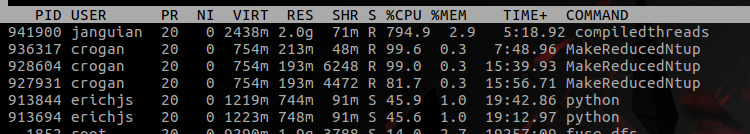
\includegraphics[scale=0.25, left]{cpusage.png}\\
	   		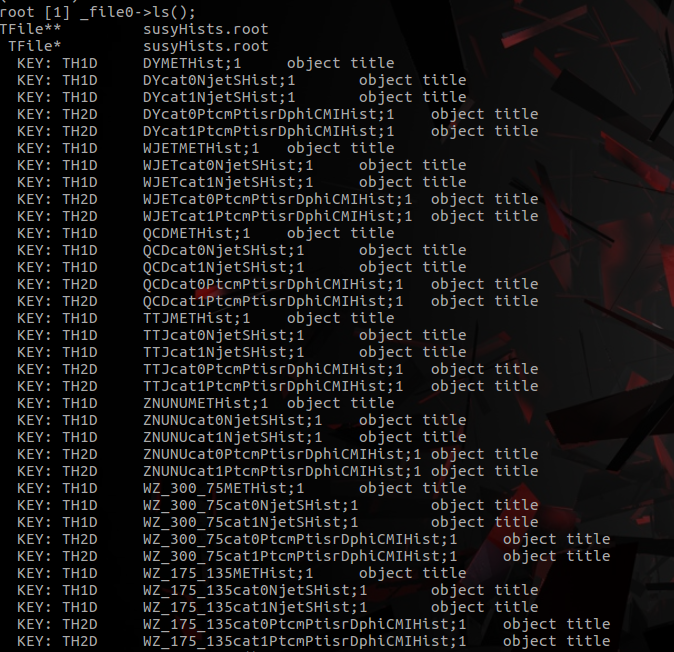
\includegraphics[scale=0.2, left]{terminaltree.png}\\
	   		\tiny
			plots produced:
			MET, Njet\_ S , PTCM/PTISR vs dPhiCMI
	\end{column}
	\begin{column}{0.5\textwidth}
		\quad \quad \\
		\quad \quad \\
		\quad \quad \\
		\quad \quad \\
			\quad \quad $Z\rightarrow \nu \nu$\\
			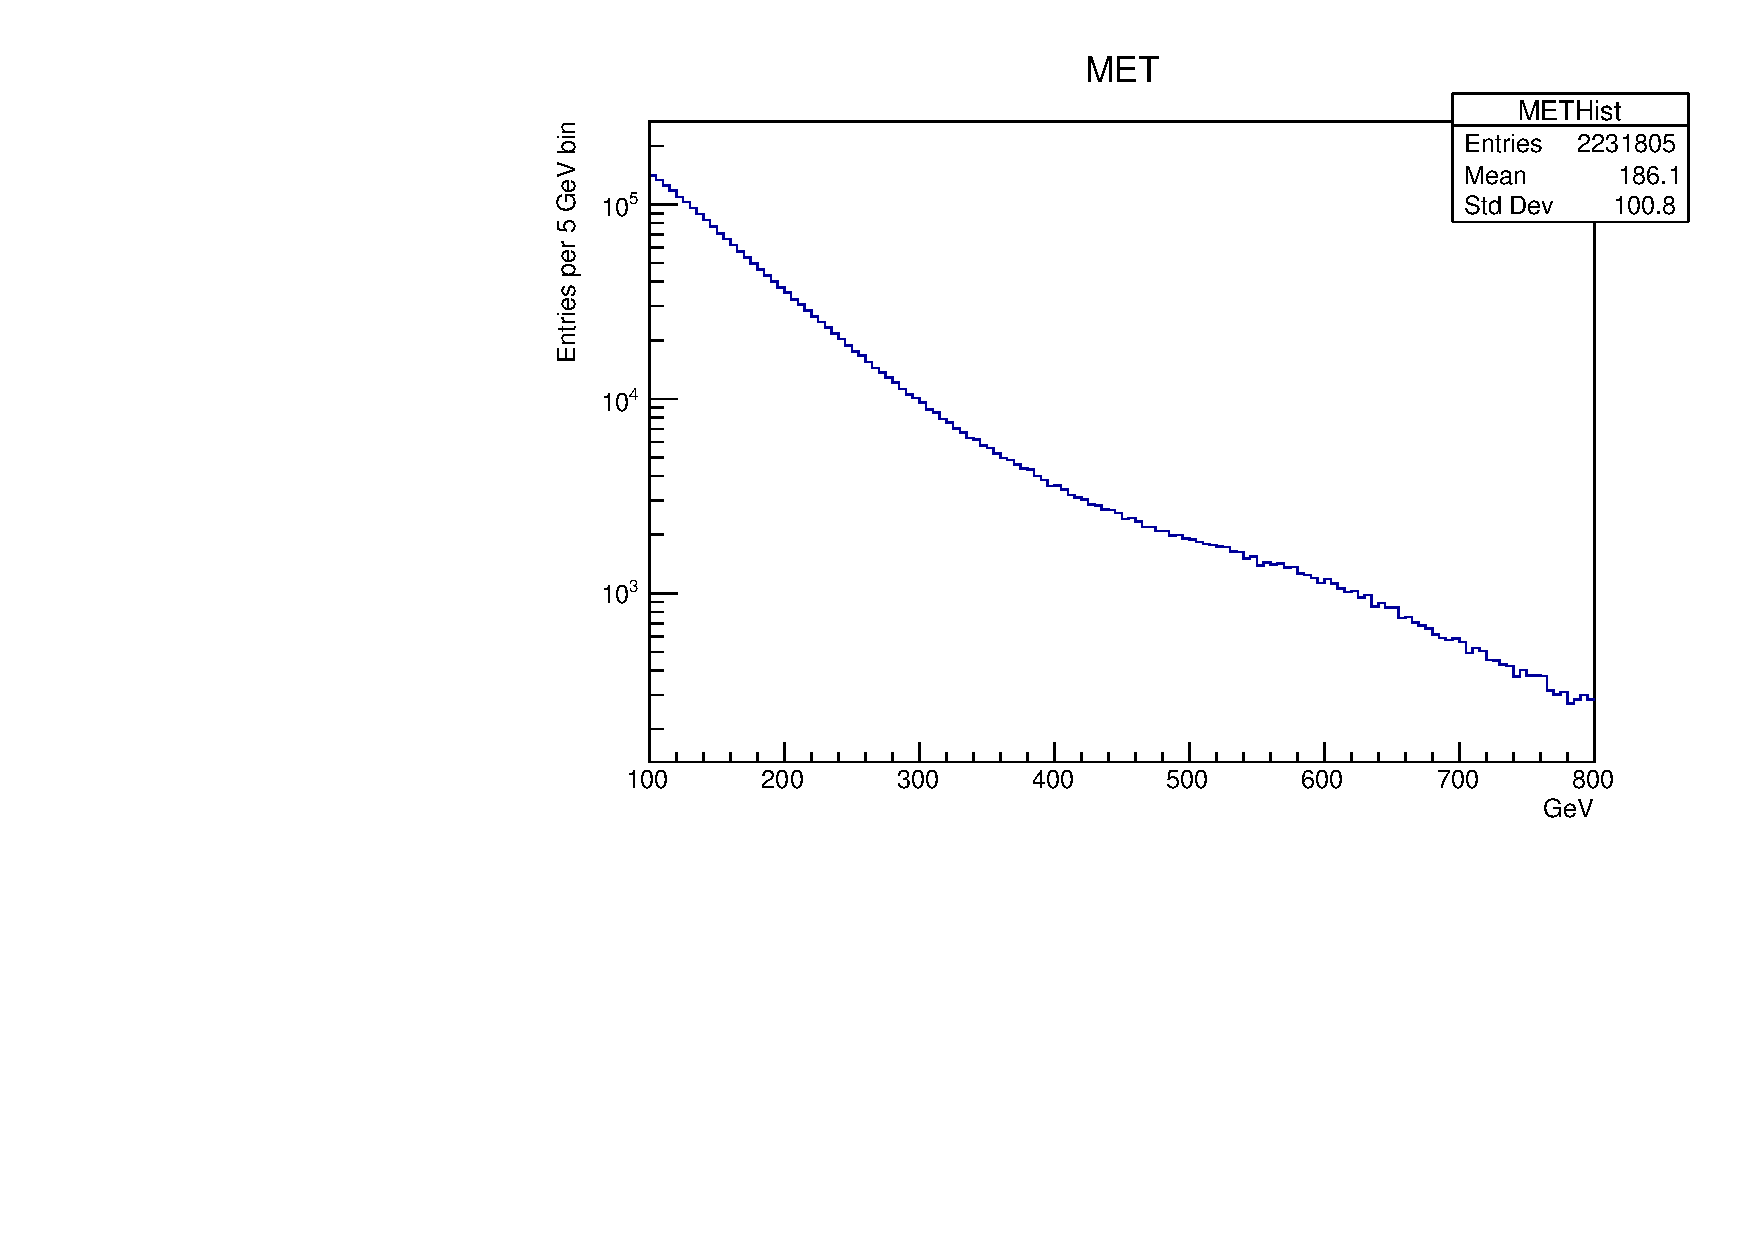
\includegraphics[scale=0.2, right]{znunuMET.pdf}\\
			\quad \quad $Z\rightarrow ll$\\
	   		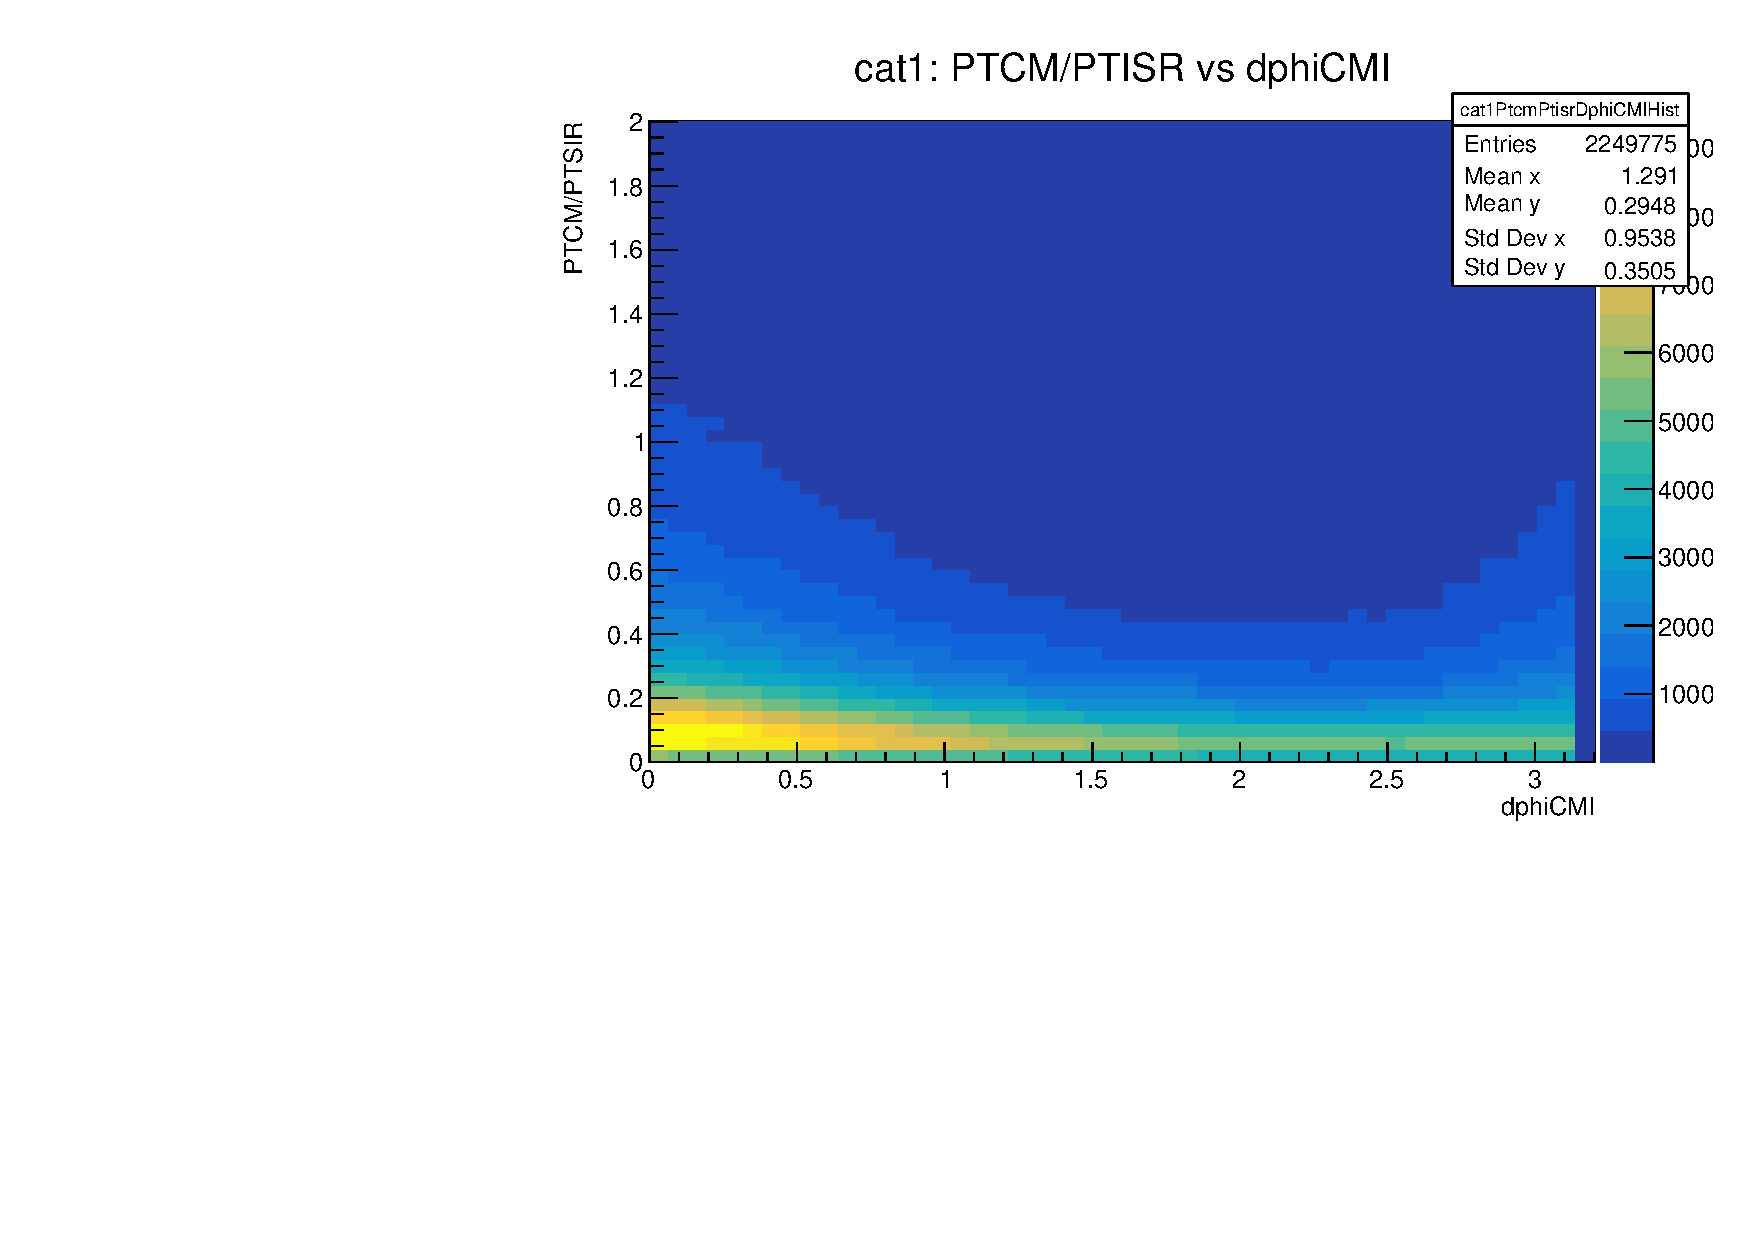
\includegraphics[scale=0.2, right]{DYdphCMI.pdf}\\
	
	\end{column}
	\end{columns}
	\scriptsize
Final Runtime: Real time-- $234.2 \pm 10.2$ s $\approx(4m)$ \quad \quad System time: $61.7 \pm 1.6$ s
\end{frame}

\begin{frame}{Conclusion}
Multithreading is very very fast! -- we need to use this --\\
\quad \quad \\
My analysis template can also be adapted to other tasks i.e. making reduced Ntuples

\quad \quad \\
Next up: Vectorization, Scientific Python - uproot etc.
\end{frame}



\end{document}